% ICRC-2021 
% Deadline 5 July
% Maximum 8 pages

% Please make sure you insert your
% data according to the instructions in PoSauthmanual.pdf
\documentclass[a4paper,11pt]{article}
\usepackage{pos} 

\usepackage[utf8]{inputenc} % Включаем поддержку UTF8
\usepackage[T2A]{fontenc}
\usepackage[russian,english]{babel}   % убрать русский перед отправкой статьи % влияет на язык подписей к рисункам и таблицам
\usepackage[modulo]{lineno}
\usepackage{graphicx}
\graphicspath{figs/}
%\usepackage[pdftex, backref, colorlinks]{hyperref}
\usepackage{todonotes}
%http://ctan.math.washington.edu/tex-archive/macros/latex/contrib/easy-todo/easy-todo.pdf
%\usepackage[enable]{easy-todo}



\title{A drone-borne installation for studying the composition of cosmic rays in the range of 1--1000~PeV by registering the reflected Cherenkov light of EAS.}
\ShortTitle{SPHERE-3 project} 

%\date{June 2021}
\author*[a,b]{I. A. Vaiman}
\author[b]{D. V. Chernov}
\author[b]{E. A. Bonvech}
\author[c,d]{M. Finger}
\author[c,d]{M. Finger Jr}
\author[a,b]{V. I. Galkin}
\author[a]{V. A. Ivanov}
\author[a]{V. S. Latypova}
\author[a,b]{D. A. Podgrudkov}
\author[b]{T. M. Roganova}

\affiliation[a]{Faculty of physics, Lomonosov Moscow State University,\\Lininskie gory, 1, Moscow, Russia}
\affiliation[b]{Skobeltsyn Institute for Nuclear Physics Lomonosov Moscow State University,\\Lininskie gory, 1, Moscow, Russia}
\affiliation[c]{Faculty of Mathematics and Physics, Charles University,\\18000 Prague, Czech Republic}
\affiliation[d]{Joint Institute for Nuclear Research,\\Dubna, Russian Federation}

\emailAdd{gosha.vaiman@gmail.com}
\emailAdd{chr@dec1.sinp.msu.ru}
\emailAdd{bonvech@yandex.ru}
\emailAdd{michael.finger@cern.ch}
\emailAdd{miroslav.finger@cern.ch}
\emailAdd{v\_i\_galkin@mail.ru}
\emailAdd{ivanov.va18@physics.msu.ru}
\emailAdd{2000vi0501g@mail.ru}
\emailAdd{d.a.podgrudkov@physics.msu.ru}
\emailAdd{rogatm@yandex.ru}

\abstract{
Here we present the current technical design of the SPHERE project’s new detector. The SPHERE project is aimed at primary cosmic ray studies in the 1--1000 PeV energy range using reflected Cherenkov light. The concept of a drone-mounted detector with a photosensitive camera based on silicon photomultipliers is discussed. The combination of the reflected CL registration method with specific data analysis approaches is a unique feature of this project. The developed earlier event-by-event data analysis approach allows to carry out primary particle mass reconstruction and PCR mass composition studies with high accuracy. This is achieved through careful analysis of each EAS CL lateral distribution function without building any kind of intermediate distributions of any `typical' characteristics.
}

\FullConference{37$^{\rm{th}}$ International Cosmic Ray Conference (ICRC 2021)\\
		July 12th -- 23rd, 2021\\
		Online -- Berlin, Germany} 

%\keywords{EAS, Cherenkov light, detector, proposal}


\begin{document}

\newcommand{\todoi}[1]{\todo[inline]{ #1}}

\linenumbers
\maketitle

\listoftodos[Notes]
\tableofcontents

\section{Introduction}

The experimental technique of detecting of the reflected Vavilov--Cherenkov radiation from extensive air showers has been known since the 70s of the last century when it was proposed by Russian academician Alexander Chudakov~\cite{chu74:VKKL74}, whose centenary is celebrated this year. 

\todoi{Написать введение. (Бонвеч)}

Ссылка на Чудакова, его 100 летие. Про метод (ЭЧАЯ).
Про проект СФЕРА. Ссылка на СФЕРУ-1. 
Помянуть "успехи" СФЕРЫ-2. Написать в духе "продолжение и развитие". (Бонвеч)

\begin{figure}
    \centering
    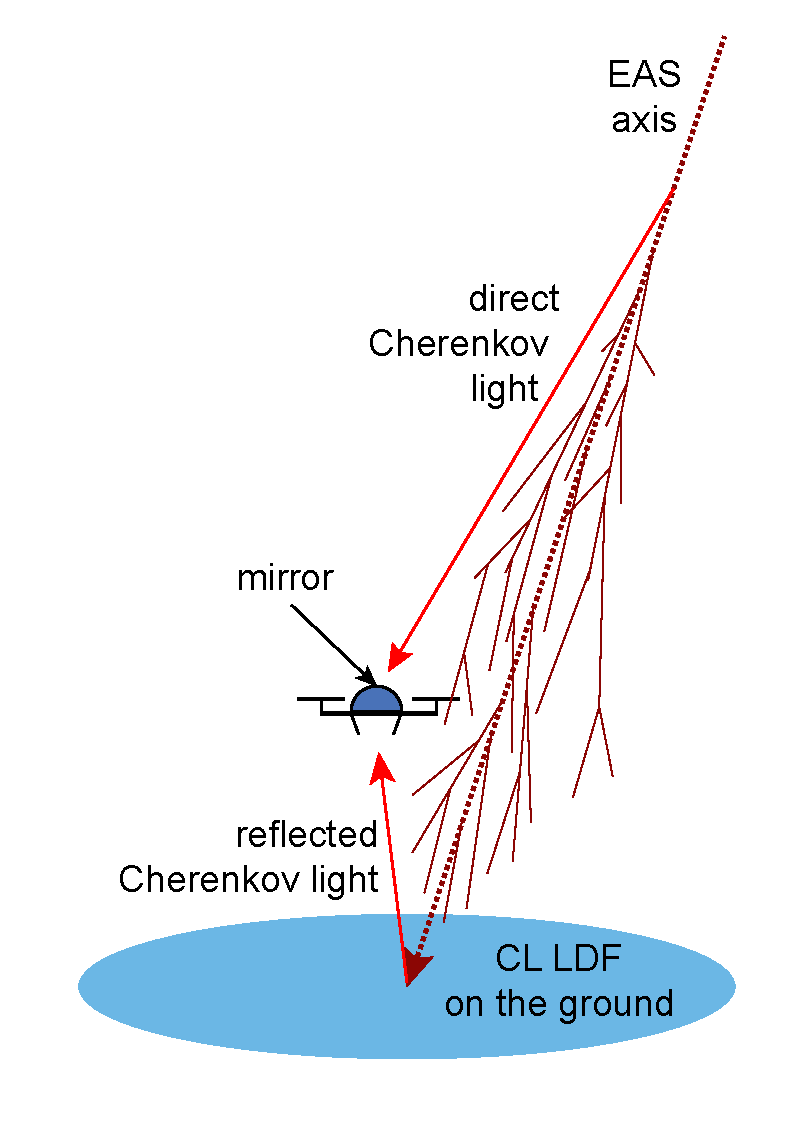
\includegraphics[width=.3\textwidth]{figs/DirectCL.pdf}
    \caption{The registration method scheme.}
    \label{fig:overview}
\end{figure}

\section{Registration method}

The general idea of the SPHERE experiment is discussed: basic idea of reflected Cherenkov light registration method and it's previous implementations in the SPHERE experiment, as well as possible additions to the method that enhance its accuracy and sensitivity.

Cherenkov light, emitted when high-energy particles travel through a medium, has long been known as an important EAS registration channel. In particular, Cherenkov light lateral distribution is indicative of the shower development details and can be used to infer both the energy and the mass of the primary particle \citep[e.g.][]{Budnev2013}.

\subsection{Reflected CL}

In the SPHERE experiment Cherenkov light is observed indirectly, after it is reflected from the `screen'. In previous SPHERE experiments, the snowfields of Antarctica and the snow-covered ice of Lake Baikal played the role of such screen. Snow has many desirable qualities in this respect, including a high overall albedo (up to $95\%$) and an almost isotropic bidirectional reflectance distribution \citep{Warren1982}.

To observe reflected Cherenkov light, a compact detector is lifted above the snow surface. The detector employs Schmidt camera technique and consists of a spherical mirror with a mosaic of sensitive elements near its focal surface. In previout SPHERE implementations detectors were lifted by a balloon to an altitude of $400$ -- $1000$~m and photomultipier tubes (PMT) served as sensititve elements. In the present paper we discuss the development of the method with a drone (UAV) as a lifting apparatus and a silicon photomultipliers (SiPM) as sensitive elements. This proposed technique is illustrated on Figure.~\ref{fig:overview}.

The optical schema of the experiment results in each sensitive element receiving light from a certain solid angle, which, in turn, correspond to a certain area on the ground. This correspondence is established on event-by-event basis, given momentary position and oriantation of the detector. We term the area of the surface, observed by a particular sensitive element it's field of view (FOV). An analogy can be drawn with a ground array technique for direct EAS Cherenkov light detection like the one used in the Tunka experiment \citep{Berezhnev2012}. Each sensitive element's FOV is analogous to a single detector in the array and the combined FOV of the mosaic is analogous to the entire array. The main difference between the two cases is the size of the detectors/FOV relative to the distance between them: in the SPHERE experiment the FOV is typically $10$ -- $100$~m in diameter depending on detector altitude, which is comparable or even greater than the distance between the centers of two adjacent FOVs and in fact adjacent FOVs almost always overlap. This means that SPHERE detector doesn't sample CL LDF at scattered points, but measures its integrals over relatively large areas, with each point within the detector's overall FOV contributing to at least one such integral. Thus, the SPHERE detector is sensitive to the near-axis region of the shower, which ground array detectors are incapable of.

% opportunities for improved precision of Cherenkov light lateral distribution reconstruction


\subsection{Direct CL}

Since the central part of the mirror is almost always shadowed by the mosaic and has little value for the light collection it can be used for different purpose.

The SPHERE-2 detector data contained the registered events from the direct Cherenkov light that got to the detector sensitive element through the gaps between mirror segments. One particular `frame' (2012-3-03559) contained both bright direct and bright reflected Cherenkov light separated by a certain amount of time. Few contained direct CL and faint image of the reflected CL (for example, 2013-3-11638). In case of SPHERE-2 detector the failure of the mirror sheath to stop direct CL was an unwanted situation resulting in more background being registered which in turn required some efforts to filter it out.

However, in gamma-astronomy the direct Cherenkov light is put to good use. In this project we propose to register direct Cherenkov light by the detector and use obtained data in the analysis. For this purpose the mirror will be turned into a coded aperture for incoming direct Cherenkov light while retaining its reflective properties for registration of reflected Cherenkov light. The accurate selection of the aperture will allow reconstruction of the direct light arrival direction (that is different from EAS arrival direction). In specific cases (near axis cases) the angular distribution of the Cherenkov light at detector level should also be accessible though registered data.

A single data point with relatively low angular distribution does not provide much data on primary particle energy and type on its own. But since the direct CL will be registered by the same sensitive element within same `frame' the precision of time measurements is expected be up to 3--5 ns. This timing information will significantly increase the precision of the primary particle arrival direction since the delay between the arrivals of the direct and reflected CL strongly depend on the EAS zenith angle. The measured total flux of the direct CL can also provide constrains on the primary particle energy and axis location. In combination with CL LDF reconstructed from the reflected CL the direct CL form data for the primary particle mass estimation hybrid criteria.

In minimal implementation of this method the mirror is planned to have a pattern of 1~cm$^2$ holes that are central projections of the pixel centers onto the mirror. Since the detector camera is offset from the focal position of the mirror the flat projection of this pattern back to the camera will be unique for every angle with respect to the variation of the sensitivity across the effective pixel. This in turn will allow reconstruction of the direct CL angular distribution.

Another option is to fill the holes in the mirror with lenses in them to focus light exactly at the camera surface. The detector in this version has limited sensitivity to the angular distribution but is more sensitive the the arrival direction of the direct CL.

More options are planned to be evaluated later in the project development.

\section{The detector}
\subsection{Detector design}
The detector is a simplified Schmidt scheme telescope without a corrector plate. The addition of the corrector plate on one hand adds more complexity to mechanical design and additional weight, on the other hand it reduces spherical aberration of the mirror. However, the proposed detector designed benefits from the relatively large light spot on its sensitive element. Therefore, the scheme without 
spherical aberration produces light spot with g
\todoi{Описание детектора (Подгрудков, Чернов)}.
\todoi{Описание оптики, электроники,... масса/зеркало/дрон. (Чернов)}
\subsection{Main drone(s)}
\todoi{Описание основного дрона (Чернов)}.
\subsection{Aux drone}
\todoi{Вспомогательный дрон. Прозрачность, контроль атмосферы.(Чернов)}
\todoi{Примеры и графики от СФЕРЫ-2. (Бонвеч)}

\section{Measurements conditions}

\subsection{Atmosphere}

Estimation of atmospheric conditions, namely its density profile, is crucial for EAS experiments, and especially for Cherenkov light modelling~\cite{Bernlhr2000}. The one advantage of air-borne detector is that it can also preform air pressure measurements which can then be used together with ground-level data to obtain information about atmosphere. Auxiliary drone can further improve the situation, providing continuous pressure measurements from the ground and beyond the detector's altitude.

The altitude of the SPHERE detector is not sufficient to fully measure even the lowest part of the atmosphere, but for 2013 SPHERE-2 measurements we used on-board pressure data to constrain possible atmosphere density profiles, given the set of standard profiles from CORSIKA \citep{CORSIKA}.

\todoi{Идея о том, что атмосфера динамична и её нужно промерять постоянно, она меняется от полёта к полёту}
\todoi{Картинка с измерениями (tele pic. 17)}
\todoi{Картинка с ФПР ЧС при нескольких разных атмосферах из набора подходящих к точкам (tele pic. 20-21)}

% * Написать про важность контроля -- ссылки на работы про это поискать. 
% * Уникальная возможность измерять состояние нижнего слоя атмосферы прямо на самой установке.
% * Возможность использования вспомогательных дронов

\subsection{Surface properties}

\todoi{Описание работы с ровным/неровным снегом, проверка отражающей способности, чем можно. (Чернов)}

\section{Analysis methods}
\subsection{CL LDF reconstruction}
\todoi{Деконволюция, режим сканирования (Подгрудков, Вайман)}

\subsection{Axis, angles, energy}
\todoi{Определение сигнала, оси и пр. (Подгрудков, Вайман)}
\subsection{Primary type}
\todoi{Методика разделения типов первичных частиц (Латыпова, Галкин).}

%Modeling procedure generally follows the approach used in SPHERE-2 experiment. It includes event modeling and image processing.
%Event modeling incorporates two stages: a) EAS simulation with CORSIKA code including Cherenkov light generation and b) the production of CL images of EAS events in the telescope mosaic. The 1st stage results in a detailed 3D-array of CL photoelecton distribution in coordinates and time delay on the snow for each EAS event. Photoelectons appear due to a special CORSIKA mode enabling account for the PMT efficiency during the shower modeling. At the 2nd stage the shower cores on the snow are evenly spread over a circle of 500 m radius centered under the telescope. Contributions to the mosaic PMTs from every patch of the CL spot on the snow are calculated on photoelectron-by-photoelectron basis.

Primary mass estimation method uses the shape of an EAS CL image in the telescope mosaic. Firstly, the images are fitted with an axisymmetric rational function. Secondly, the approximations are integrated over a central circle and the surrounding ring. Thirdly, a ratio of these integrals is used as a criterion parameter for the separation of events by the primary mass. Criteria are optimized with respect to the mass separation by varying the radii of the circle and the ring. Optimal criteria are obtained for different primary energies and zenith angles, detector elevation and atmosphere models (1 and 11 in CORSIKA terms).

One can rely on the primary energy and zenith angle estimates derived from the event data and thus use different criteria for different combinations of these primary parameters and also for different values of the detector elevation which is measurable. Atmosphere model affects the mass criteria as well and must be taken into account while processing the images.
We hope to be able to promptly register the parameters of the local atmosphere (up to at least 20 km above the snow) during the experiment. Hadron interaction at super high energies presents another problem as its different models lead to different shower behaviours. According to our experience, the use of shape characteristics as criterion parameter substantially reduces the effect of interaction model on primary mass criterion. Still, the effect must be known and the final criterion should be selected in such a way so as to minimize its dependence on the model.

One more possibility to improve the primary mass resolution is the use of the direct CL angular distribution which is proved to be a powerful instrument for this task\cite{Gal18a}.

\todoi{Про оптимизацию геометрии и критерия друг под друга. (Галкин)}
The design of the telescope and the circumstances of the experiment (such as detector elevation height) affect the mass separation procedure and the resulting primary mass resolution. As we aim at constructing a detector for the solution of the primary cosmic ray mass composition problem we have to optimize the detector design with respect to this goal. To do so we are sentenced to consider a few experiment configurations with the corresponding image processing techniques and choose the one with the best mass resolution.


\section{Discussion}
\todoi{Pro et con (all)}

\section{Conclusions}
\todoi{Выводы.}

\acknowledgments
\todoi{Гранты? (Чернов)}
M. Finger and M. Finger Jr thank MEYS of Czech Republic for grants LG14004 and LG18022.

\bibliographystyle{JHEP}
\bibliography{references}
\todoi{Ссылки. (Бонвеч)}

\end{document}
